\documentclass{article}


\usepackage{graphicx}
\usepackage[latin1]{inputenc}
\usepackage[spanish,es-tabla]{babel}

\usepackage[font=footnotesize,caption=false,farskip=0mm,captionskip=0mm,nearskip=0mm]{subfig}

\usepackage{array}
\usepackage{longtable}
\usepackage{cite}
\usepackage{supertabular}
\usepackage{anysize}
\marginsize{2.5cm}{2.5cm}{2.5cm}{2.5cm}
\usepackage{psfrag}

\usepackage[table]{xcolor}
\usepackage{color}
\usepackage[font=footnotesize,caption=false,farskip=0mm,captionskip=0mm,nearskip=0mm]{subfig}
\usepackage{dsfont}
\usepackage{amsfonts}
\usepackage{amsmath}
\usepackage{amssymb}
\usepackage{amsxtra}
\usepackage{multirow}
\usepackage{gensymb}


\usepackage{fancyhdr}
\pagestyle{fancy}
\lhead{Ayudant�a de ingenier�a de Software}
\chead{}
\rhead{2� Sem. 2013}

\hyphenation{in-te-rrup-tor}

\marginsize{2.5cm}{2.5cm}{2.5cm}{2.5cm}
%\topmargin=-1cm
\setlength{\unitlength}{1 cm} %Especificar unidad de trabajo

\begin{document}
\thispagestyle{empty}
%\begin{picture}(18,4)
%\put(0,0){\includegraphics[width=3cm,height=4cm]{uco.jpg}}
%\put(11.5,0){\includegraphics[width=4cm,height=4cm]{eupinf.jpg}}
%\end{picture}
%\\
%\\
\begin{flushleft}
\textsc{Universidad Tecnol�gica Metropolita\\Departamento de Inform�tica\\Ayudant�a de ingenier�a de Software}
\end{flushleft}
\vspace{50mm}
\begin{center}
\textbf{\Huge �gil Vs Tradicional }\\
\vspace{5mm}
\end{center}
\vspace{70mm}
\begin{flushright}

\vspace{5mm}
(\textbf{Alumnos: }Ronald Verdugo Lemus y David Martinez)\\
(\textbf{Ayudante: }Cristian Garrido)\\
\vspace{5mm}
\today
\end{flushright}

\newpage{\pagestyle{empty}\cleardoublepage}

\begin{enumerate}
\item \textbf{(Comparativa �gil Vs Tradicional)}\\

\vspace{10cm}
\begin{figure}[h]
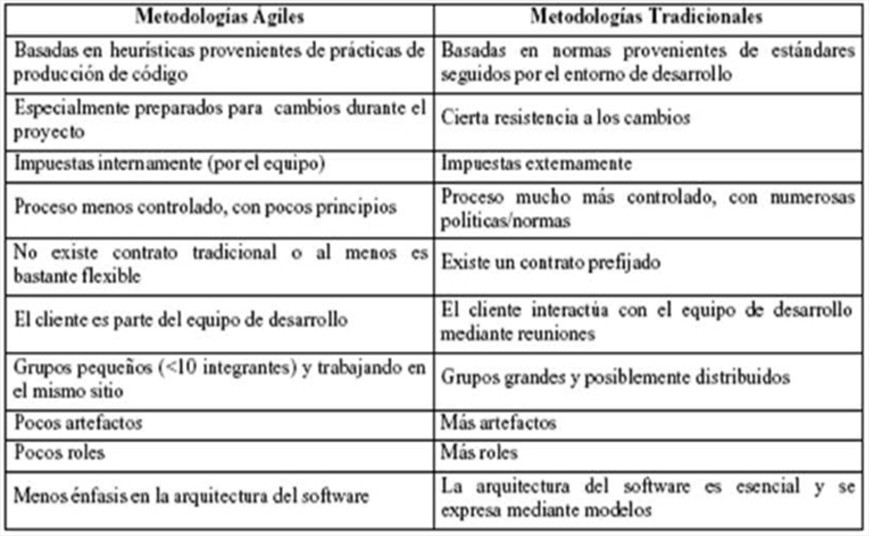
\includegraphics[width=38pt]{agil_vs_tradicional.jpg}
\end{figure}
\item \textbf{Como res�men, existen dos grandes conclusiones:}\\

\begin{itemize}
	\item No hay varitas m�gicas para conseguir mejorar la calidad y rendimiento de los equipos de manera radical sin cambiar profundamente la manera de trabajar. Y esto no supone en absoluto que los cambios sean dif�ciles si la direcci�n y los miembros de la organizaci�n creen en ello decididamente.

\end{itemize}

\begin{itemize}
	\item Cada organizaci�n en mundo. Aplicar una metodolog�a est�ndar de manera r�pida y sin trabajar abierta y reflexivamente con los miembros de un equipo suele ser una buena receta para el desastre.
\end{itemize}

\item \textbf{(https://github.com/ronaldvl/AyudantiaSw Tareas)}\\

\end{document}
\end{enumerate}
\end{document} 